\documentclass[11pt]{article}
\usepackage[margin=2.5cm]{geometry}
\usepackage[utf8]{inputenc}
\usepackage[T1]{fontenc}
\usepackage[spanish,es-tabla]{babel}
\usepackage{graphicx}
\usepackage{float}
\usepackage{booktabs}
\usepackage{array}
\usepackage{caption}
\usepackage{subcaption}
\usepackage{hyperref}
\usepackage{longtable}
\usepackage{enumitem}
\usepackage{amsmath}
\usepackage{amssymb}

\hypersetup{
  colorlinks=true,
  linkcolor=black,
  urlcolor=blue
}

\title{Laboratorio 1: Series de Tiempo\\Análisis de viajeros internacionales a Guatemala}
\author{Pablo Méndez \\ María José Yee}
\date{\today}

\begin{document}

\maketitle
\tableofcontents
\newpage

\section{Introducción}

Este informe documenta la resolución de los ejercicios 1 al 5 del laboratorio de series de tiempo utilizando los datos de ingreso mensual de viajeros internacionales a Guatemala entre 2009 y junio de 2026. Se emplearon herramientas de Python para la carga, limpieza, visualización, detección de valores atípicos, descomposición temporal y comparación de modelos predictivos.

Los resultados obtenidos fueron exportados a imágenes PNG que sirven de soporte visual para este reporte. El análisis se centra en tres series principales: la serie total mensual, la serie de viajeros por vía aérea y la serie de viajeros por vía terrestre.

\section{Ejercicio 1: Carga, preparación y calidad de los datos}

La base de datos original fue cargada desde el archivo Excel y se transformó a un formato adecuado para el análisis de series de tiempo. Se normalizaron los nombres de columnas, se construyó la variable de fecha mensual y se corrigieron los tipos de datos para trabajar con la variable de viajeros como numérica.

\subsection{Resumen de calidad de datos}

El conjunto de datos presentó 161036 observaciones y 14 columnas. No se detectaron filas duplicadas ni valores faltantes. La serie total mensual quedó conformada por 210 meses calendario, sin meses faltantes.

\begin{table}[H]
\centering
\caption{Resumen de calidad de los datos}
\begin{tabular}{lrrr}
\toprule
Variable & Faltantes & \% Faltantes & Unidades únicas \\
\midrule
Año & 0 & 0.00 & 18 \\
Mes & 0 & 0.00 & 12 \\
Vía & 0 & 0.00 & 3 \\
Frontera & 0 & 0.00 & 22 \\
País & 0 & 0.00 & 235 \\
Tipo de viajero & 0 & 0.00 & 4 \\
Viajero & 0 & 0.00 & 38122 \\
\bottomrule
\end{tabular}
\end{table}

\subsection{Observaciones principales}

\begin{itemize}[leftmargin=*]
  \item El periodo analizado abarca desde enero de 2009 hasta junio de 2026.
  \item El volumen total acumulado de viajeros alcanzó valores muy superiores a los reportados en los años iniciales del periodo.
  \item La mayoría de los registros corresponden a turistas y a las vías terrestre y aérea.
\end{itemize}

\section{Ejercicio 2: Análisis exploratorio de datos}

Se elaboró una exploración inicial de la serie temporal total y de las categorías más relevantes del conjunto. La figura \ref{fig:total-temporal} muestra la evolución mensual y anual del total de viajeros, mientras que la figura \ref{fig:categorias} resume las categorías con mayor participación.

\begin{figure}[H]
\centering
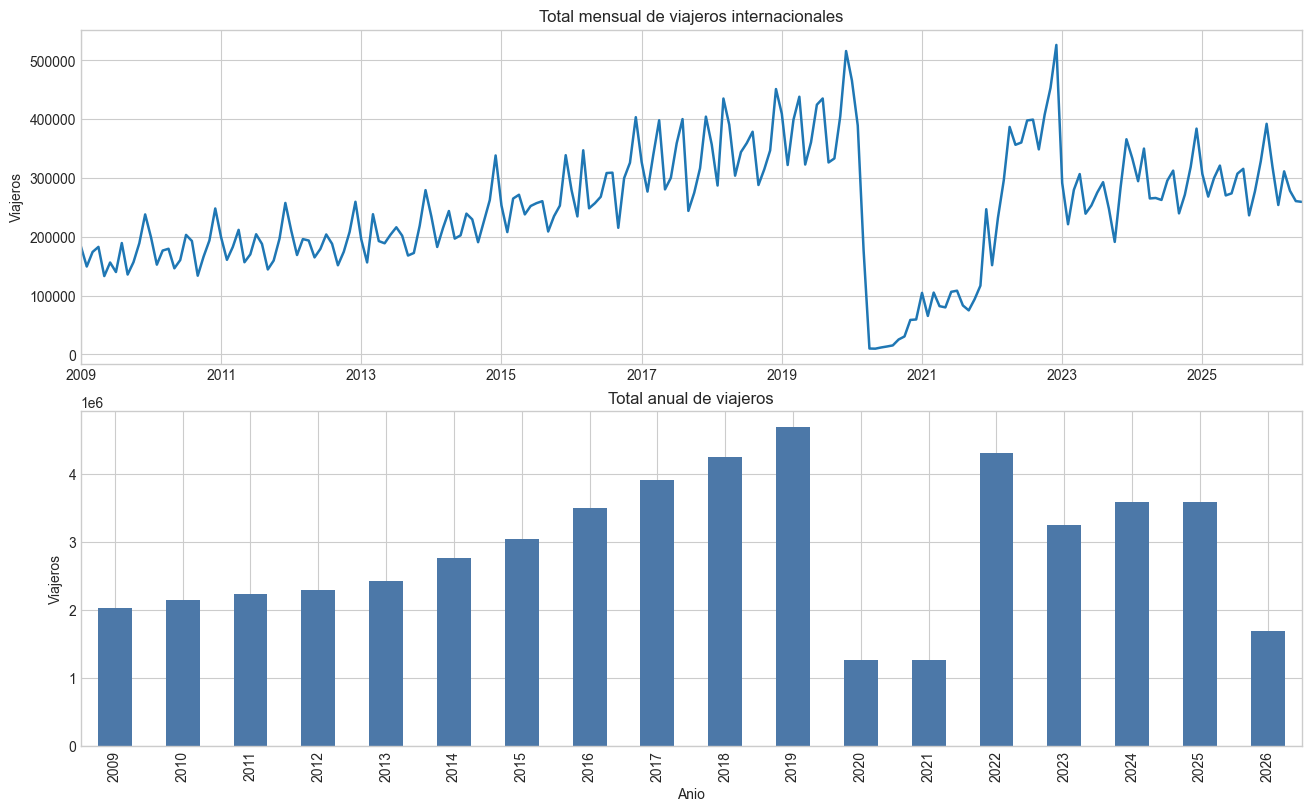
\includegraphics[width=0.95\textwidth]{01_total_temporal.png}
\caption{Serie temporal mensual y anual del total de viajeros internacionales}
\label{fig:total-temporal}
\end{figure}

\begin{figure}[H]
\centering
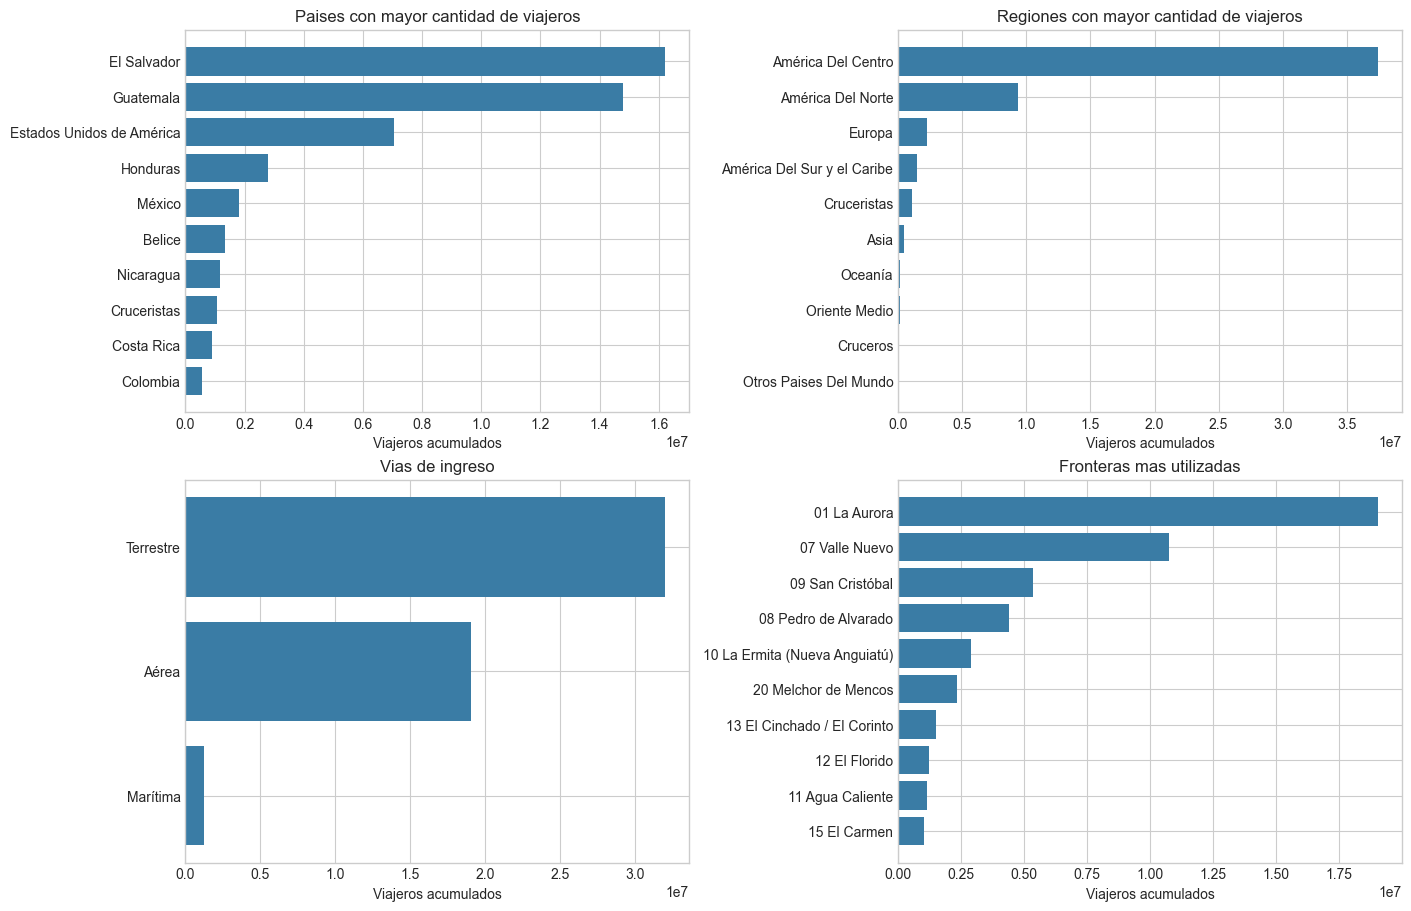
\includegraphics[width=0.95\textwidth]{02_categorias_barh.png}
\caption{Categorías con mayor contribución al total de viajeros}
\label{fig:categorias}
\end{figure}

\subsection{Hallazgos del análisis exploratorio}

\begin{itemize}[leftmargin=*]
  \item La serie total presenta crecimiento sostenido en el largo plazo, con una caída abrupta durante 2020 por efecto de la pandemia.
  \item El país con mayor participación es El Salvador, seguido de Guatemala y Estados Unidos de América.
  \item La vía terrestre concentra el mayor volumen de viajeros, con 61.19\% del total, seguida por la vía aérea con 36.46\% y la marítima con 2.35\%.
  \item Los turistas representan 71.99\% del total de viajeros analizados.
\end{itemize}

\section{Ejercicio 3: Detección de valores atípicos}

Para identificar observaciones extremas se utilizó el criterio IQR sobre la serie mensual total. La figura \ref{fig:boxplot} muestra la distribución de la serie y los potenciales valores atípicos.

\begin{figure}[H]
\centering
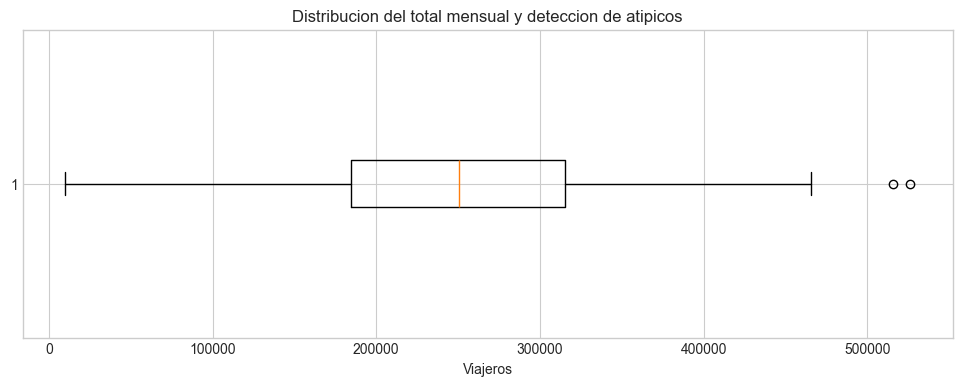
\includegraphics[width=0.9\textwidth]{03_boxplot_outliers.png}
\caption{Diagrama de caja para la detección de valores atípicos en la serie mensual total}
\label{fig:boxplot}
\end{figure}

\subsection{Resultados de la detección}

Los límites calculados mediante IQR fueron:
\begin{itemize}[leftmargin=*]
  \item Límite inferior: $-11{,}577$
  \item Límite superior: $511{,}543$
\end{itemize}

Los meses identificados como atípicos fueron diciembre de 2019 y diciembre de 2022, lo cual coincide con episodios de alta demanda en el periodo analizado.

\section{Ejercicio 4: Construcción de series mensuales y descomposición STL}

Se construyeron series mensuales para el total global y para las vías aérea y terrestre. Posteriormente se aplicó la descomposición STL para separar tendencia, estacionalidad y residuo.

\begin{figure}[H]
\centering
\begin{subfigure}{0.32\textwidth}
  \centering
  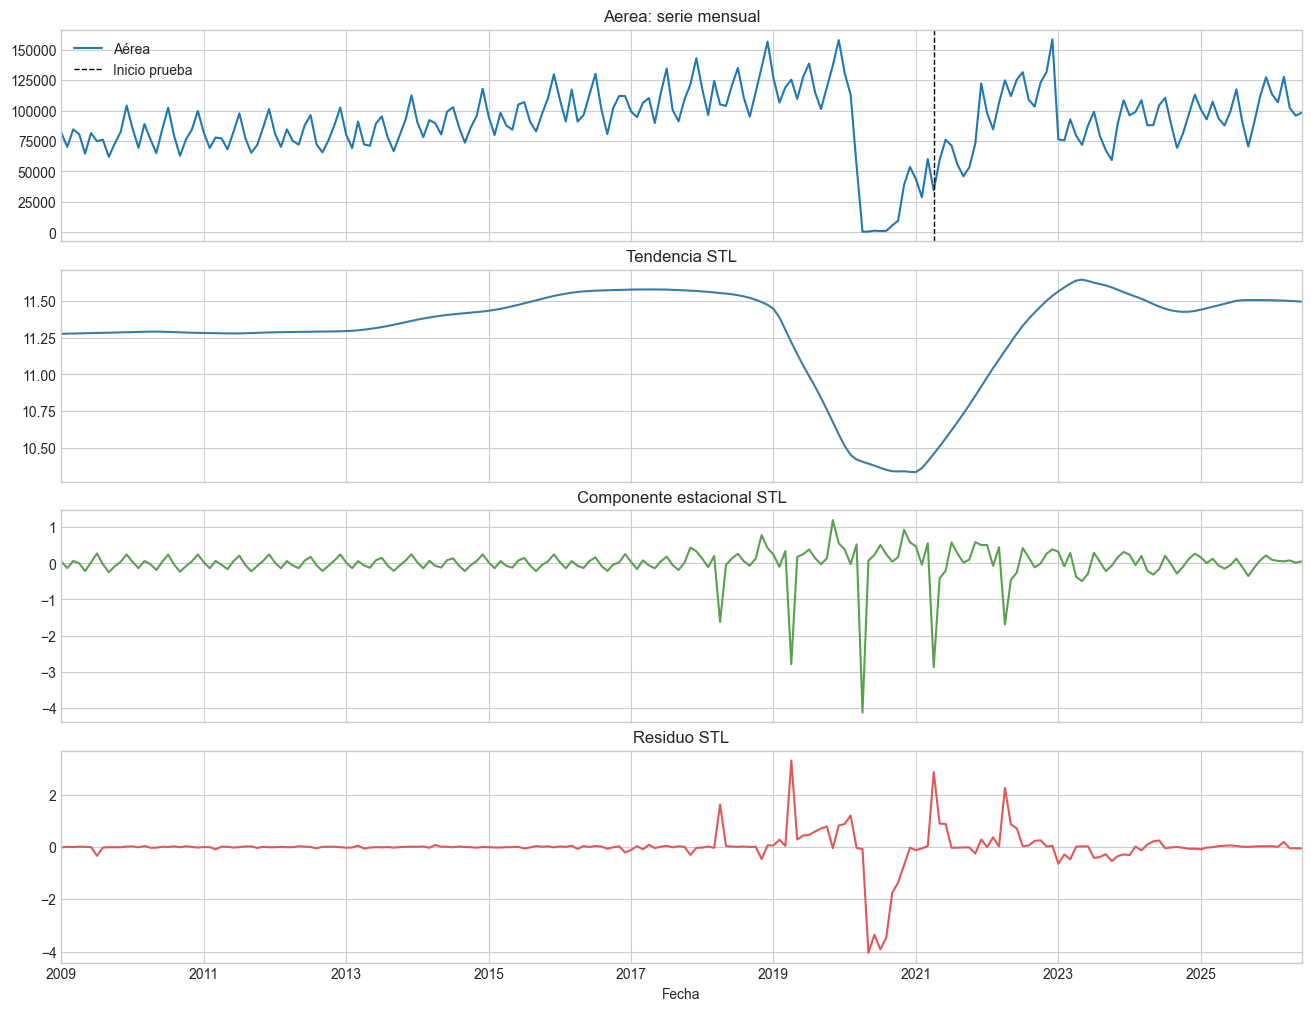
\includegraphics[width=\linewidth]{04_Aerea_descomposicion.png}
  \caption{Aérea}
\end{subfigure}
\hfill
\begin{subfigure}{0.32\textwidth}
  \centering
  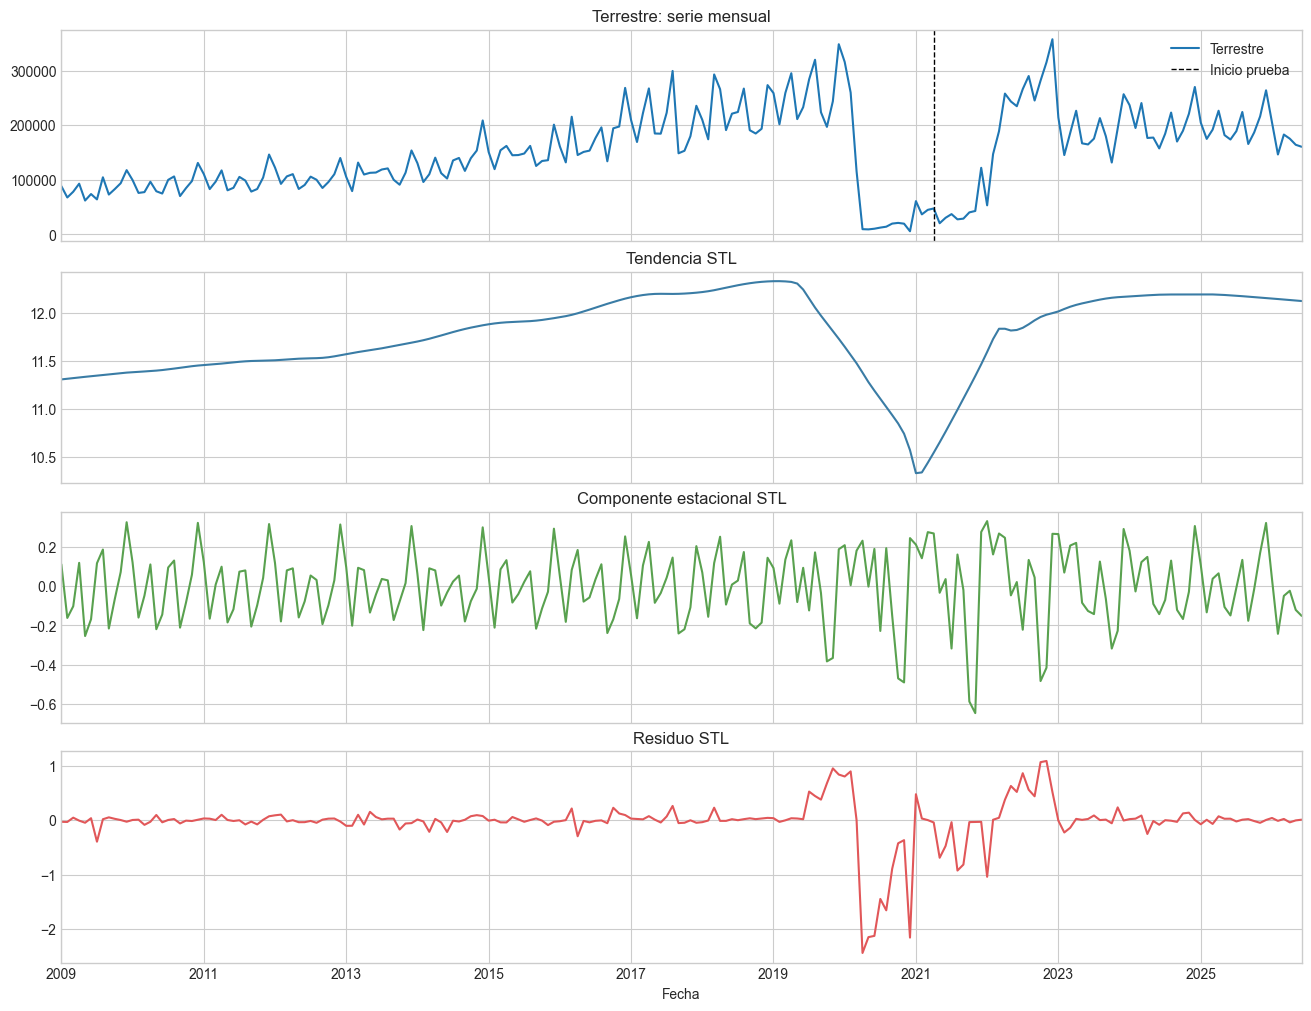
\includegraphics[width=\linewidth]{04_Terrestre_descomposicion.png}
  \caption{Terrestre}
\end{subfigure}
\hfill
\begin{subfigure}{0.32\textwidth}
  \centering
  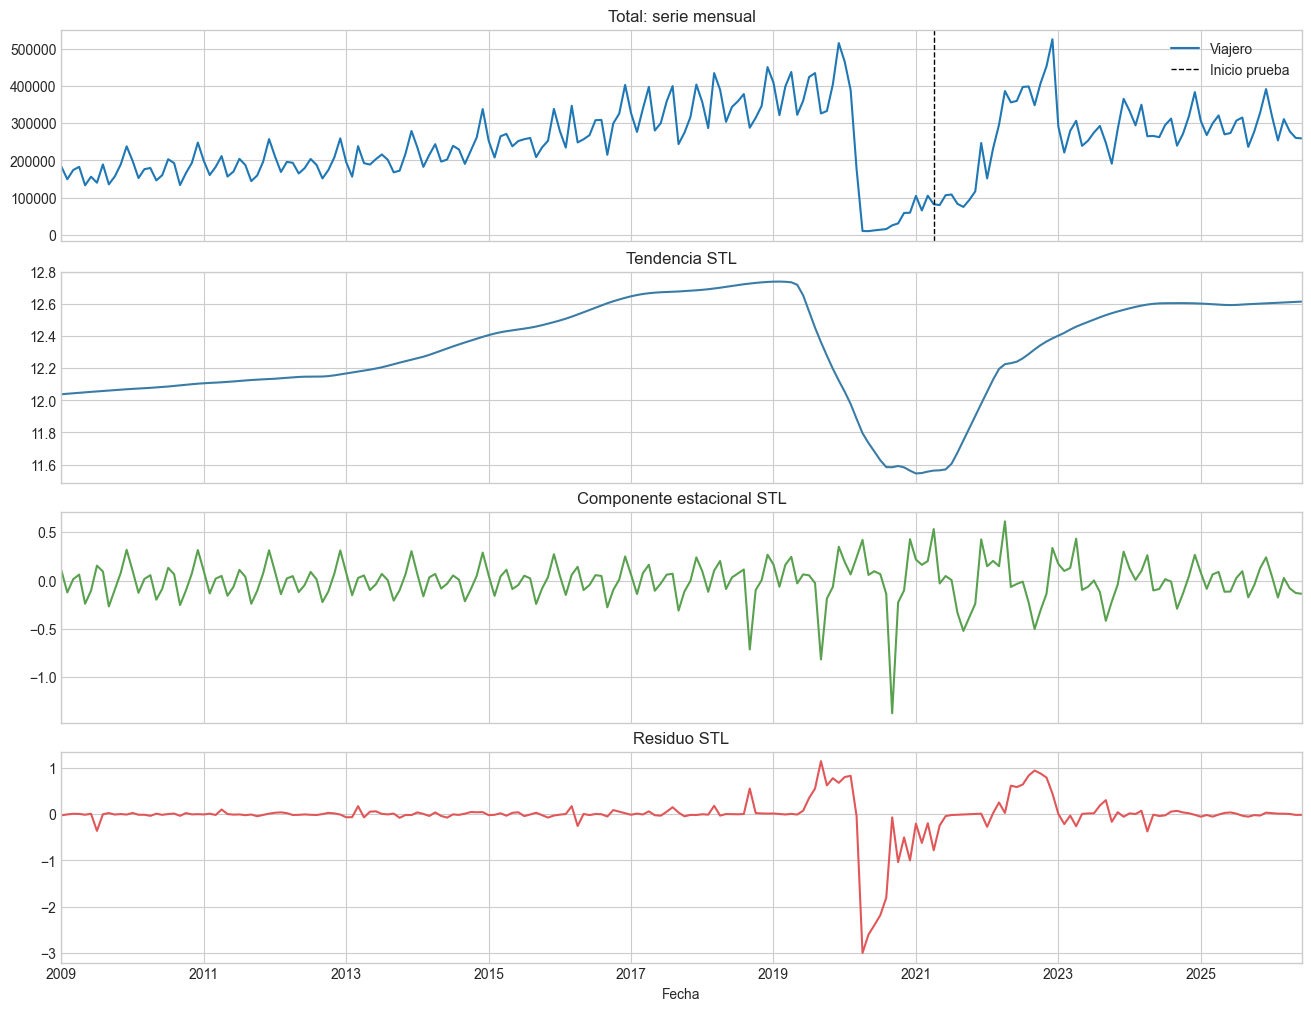
\includegraphics[width=\linewidth]{04_Total_descomposicion.png}
  \caption{Total}
\end{subfigure}
\caption{Descomposición STL de las series de viajeros por vía aérea, terrestre y total}
\label{fig:stl}
\end{figure}

\subsection{Interpretación de la descomposición}

\begin{itemize}[leftmargin=*]
  \item La serie total muestra una fuerte componente estacional y un cambio estructural en 2020.
  \item La vía aérea exhibe mayor variabilidad y mayor sensibilidad a eventos externos.
  \item La vía terrestre es la más estable en volumen, aunque también presenta un impacto claro por la pandemia.
\end{itemize}

\section{Ejercicio 5: Análisis de autocorrelación y modelos predictivos}

Se analizaron los correlogramas ACF y PACF para cada serie y se compararon diversos modelos ARIMA, suavizamiento exponencial y seasonal naive. Los resultados se muestran en las figuras \ref{fig:acf-pacf} y \ref{fig:forecast}.

\begin{figure}[H]
\centering
\begin{subfigure}{0.32\textwidth}
  \centering
  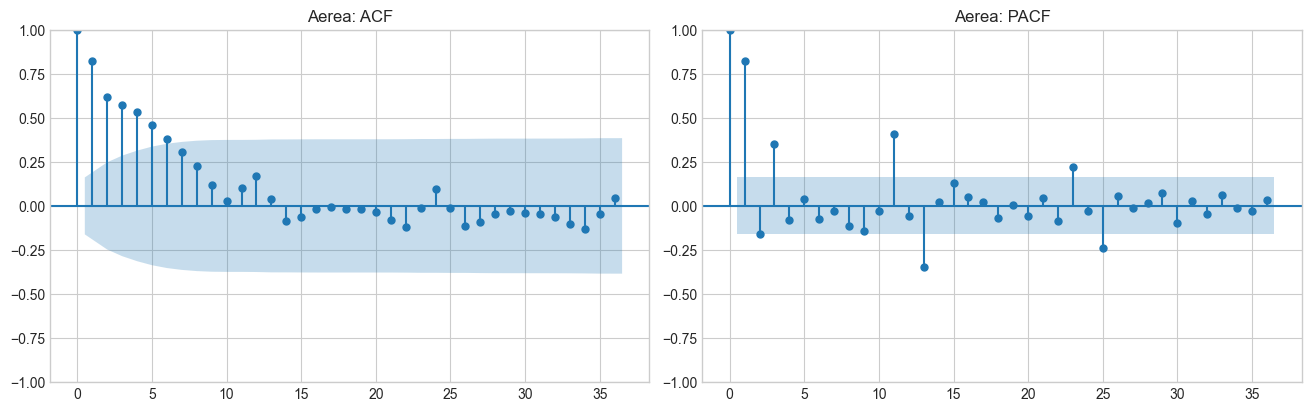
\includegraphics[width=\linewidth]{05_Aerea_acf_pacf.png}
  \caption{Aérea}
\end{subfigure}
\hfill
\begin{subfigure}{0.32\textwidth}
  \centering
  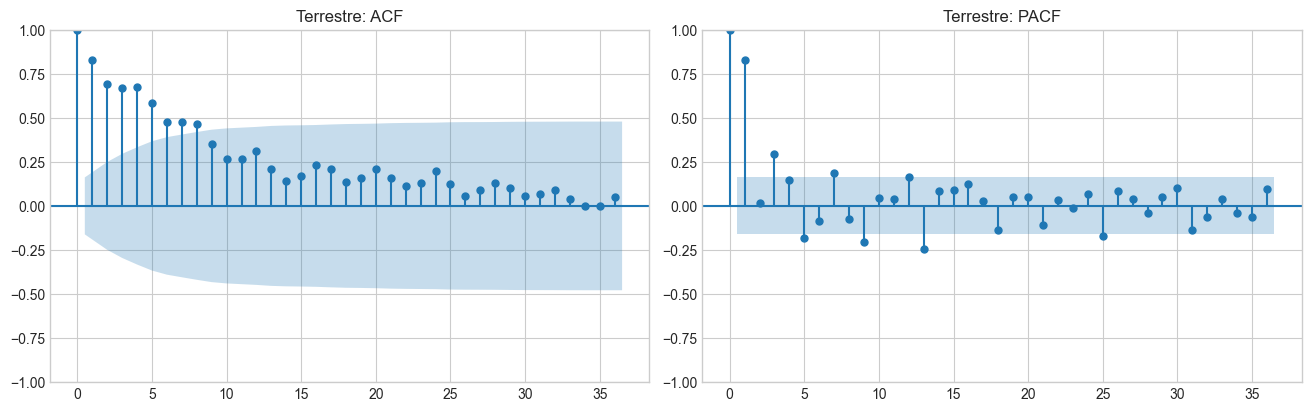
\includegraphics[width=\linewidth]{05_Terrestre_acf_pacf.png}
  \caption{Terrestre}
\end{subfigure}
\hfill
\begin{subfigure}{0.32\textwidth}
  \centering
  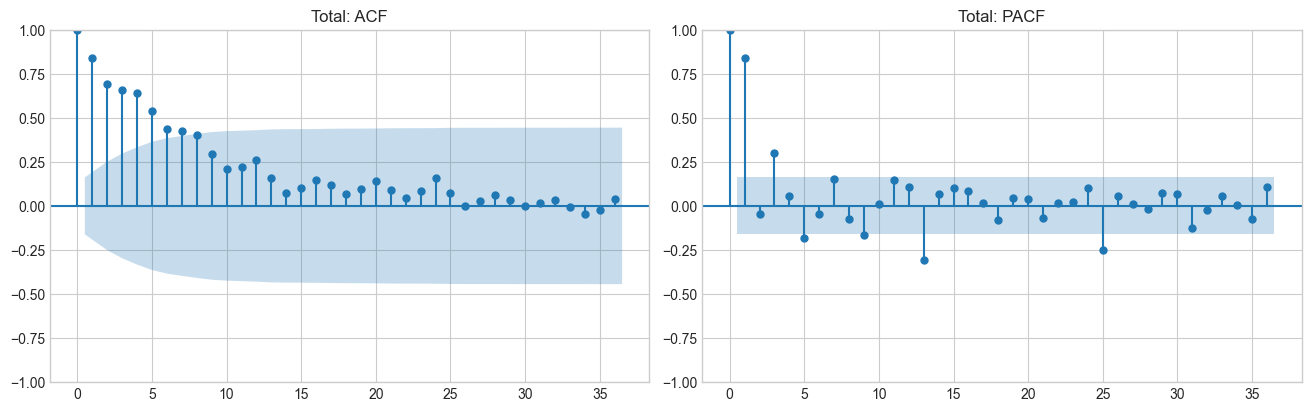
\includegraphics[width=\linewidth]{05_Total_acf_pacf.png}
  \caption{Total}
\end{subfigure}
\caption{Correlogramas ACF y PACF de las series analizadas}
\label{fig:acf-pacf}
\end{figure}

\begin{figure}[H]
\centering
\begin{subfigure}{0.32\textwidth}
  \centering
  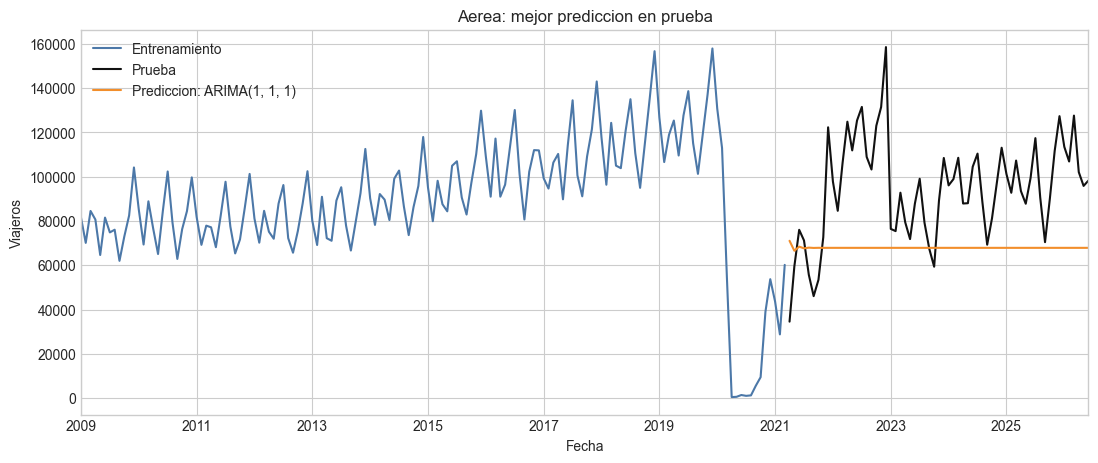
\includegraphics[width=\linewidth]{06_Aerea_mejor_prediccion.png}
  \caption{Aérea}
\end{subfigure}
\hfill
\begin{subfigure}{0.32\textwidth}
  \centering
  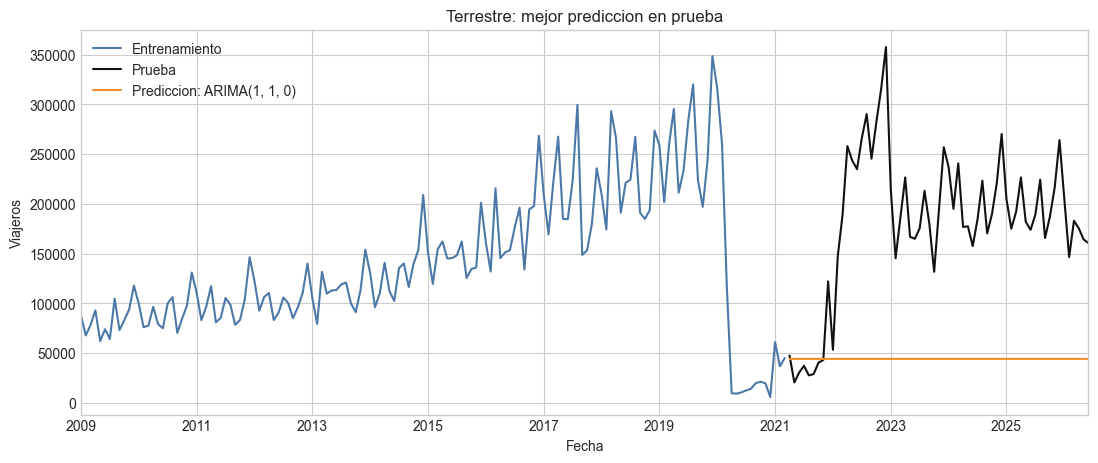
\includegraphics[width=\linewidth]{06_Terrestre_mejor_prediccion.png}
  \caption{Terrestre}
\end{subfigure}
\hfill
\begin{subfigure}{0.32\textwidth}
  \centering
  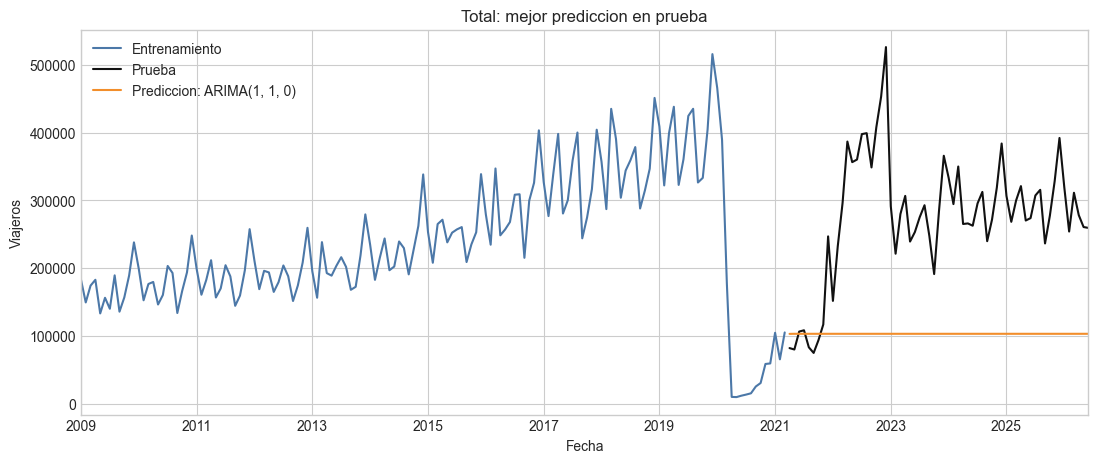
\includegraphics[width=\linewidth]{06_Total_mejor_prediccion.png}
  \caption{Total}
\end{subfigure}
\caption{Comparación entre la serie real y la mejor predicción obtenida}
\label{fig:forecast}
\end{figure}

\begin{table}[H]
\centering
\caption{Modelos con menor error RMSE por serie}
\begin{tabular}{lcc}
\toprule
Serie & Mejor modelo & RMSE \\
\midrule
Total & ARIMA(1,1,0) & 196,552.53 \\
Aérea & ARIMA(1,1,1) & 35,269.52 \\
Terrestre & ARIMA(1,1,0) & 155,420.18 \\
\bottomrule
\end{tabular}
\end{table}

\subsection{Conclusiones del ejercicio 5}

\begin{itemize}[leftmargin=*]
  \item Los mejores modelos para las series evaluadas fueron modelos ARIMA con diferenciación de primer orden.
  \item La serie aérea mostró mayor sensibilidad a la estructura temporal y un mejor ajuste con el modelo ARIMA(1,1,1).
  \item La serie total y la terrestre fueron bien ajustadas mediante ARIMA(1,1,0).
  \item La comparación de predicciones confirmó que los modelos capturan de manera razonable el comportamiento general de las series, aunque la incertidumbre aumenta en periodos de cambio estructural.
\end{itemize}

\section{Conclusiones generales}

El laboratorio permitió validar la importancia de la preparación de datos, la visualización exploratoria y el uso de métodos estadísticos para comprender series de tiempo. En particular, la caída de 2020 evidenció que los eventos externos pueden modificar de manera sustancial la estructura de una serie. Asimismo, los modelos ARIMA seleccionados demostraron ser adecuados para generar predicciones cortas y representar el comportamiento general de las series analizadas.

\section{Anexo: Figura comparativa}

\begin{figure}[H]
\centering
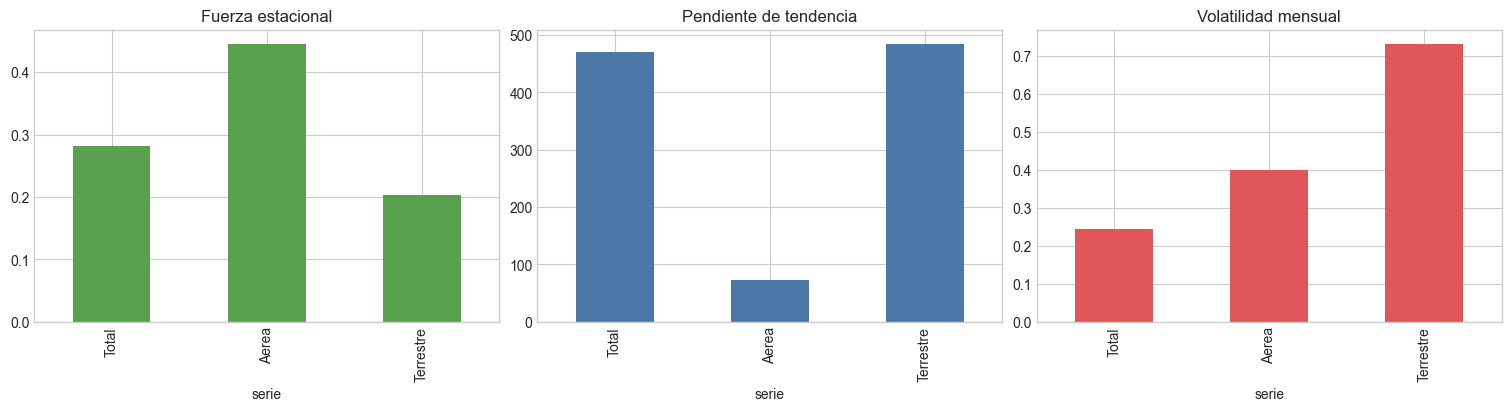
\includegraphics[width=0.95\textwidth]{07_comparacion_series.png}
\caption{Comparación estadística entre las series de total, aérea y terrestre}
\end{figure}

\end{document}
